\documentclass[letterpaper, reqno,11pt]{article}
\usepackage[margin=1.0in]{geometry}
\usepackage{color,latexsym,amsmath,amssymb,graphicx,float,listings,tikz}
\usepackage{hyperref}

\hypersetup{
colorlinks=true,
linkcolor=magenta,
filecolor=magenta,
urlcolor=cyan,
}

\graphicspath{ {images/} }

\begin{document}
\pagenumbering{arabic}
\title{Math 406 Homework 1}
\date{27/09/23}
\author{Xander Naumenko}
\maketitle

{\medskip\noindent\bf Question 1a.} Let the best fit polynomial be $p(x)=p_0+p_1x+\cdots+p_mx^{m}$, then the value of $p$ at each point $x_n$ is:
\[
    \begin{pmatrix} 1&x_1&x_1^2\ldots x_N^{m}\\ \vdots\\ 1&x_N&x_N^2\ldots x_N^{m}\end{pmatrix} \begin{pmatrix} p_0\\\vdots \\p_m \end{pmatrix} =Ay
.\]
The value of the points is $b=\begin{pmatrix} f(x_1)\\ \vdots \\f(x_N) \end{pmatrix} $, so the system we are trying to minimize is:
\[
|Ax-b|^2
.\]
From linear algebra, for this to be minimized $Ay-b$ is in the null space of $A$, i.e. $A^{t}(Ay-b)=0$. Rewriting this, we get the system of equations to solve:
\[
A^{t}Ay=A^{t}b
.\]
The size of the matrix $A^{t}A$ is $(m+1)\times (m+1)$.

{\medskip\noindent\bf Question 1b.} The matlab operator ``\textbackslash'' solves least square problems automatically, so this was used to get the coefficients. Using the code, the approximation for $x=0.5$ was $0.3582$ and $0.359573$, compared with the real value of $0.359569$. The coefficients found with this method matched those found with polyfit. The code used was as follows:
\begin{lstlisting}
m = 5;

x = [0, 0.2, 0.3, 0.4, 0.6, 1];
A = x(:).^(0:1:m);
b = (1-x.^2).*sin(x);
y = A \ b';

display((0.5.^(0:1:m))*y)
display((1-0.5^2).*sin(0.5))

polyfit(x, b, m)
\end{lstlisting}

The fits were for $m=3$:

\begin{lstlisting}
y =-0.0004
    1.0509
   -0.2844
   -0.7662
\end{lstlisting}

For $m=5$:

\begin{lstlisting}
y = 0
    0.9997
    0.0038
   -1.1851
    0.0390
    0.1425
\end{lstlisting}

{\medskip\noindent\bf Question 2.} Here is the matlab code used:
\begin{lstlisting}
forwarddiff(5)

function s = ksum(N, k)
    s = sum((1:N).^k);
end

function t = forwarddiff(k)
    t = zeros(k+3, k+1);
    
    t(:, 1) = arrayfun(@(x) ksum(x, k), 1:k+3);
    
    for j = 2:(k+3)
        for i = 1:(k+3-j+1)
            t(i, j) = t(i+1, j-1) - t(i, j-1);
        end
    end
    t = t';
end
\end{lstlisting}

This produced the following difference table:
\begin{lstlisting}
   1    33    276  1300  4425  12201  29008  61776
  32   243   1024  3125  7776  16807  32768
 211   781   2101  4651  9031  15961
 570  1320   2550  4380  6930
 750  1230   1830  2550
 480   600    720
 120   120
   0
\end{lstlisting}

Thus $\Delta^{6} S_N^{k}=0$. To see why this always terminates for all $k$, note that $\Delta S_N^{k}=x^{N+1}$, which is a polynomial. For any polynomial $p(x)=p_m x^{m}+\ldots p_0$, note that $p(x+1)-p(x)$ is a polynomial of degree $m-1$. Thus differencing further terms of $S_N^{k}$ polynomials of strictly decreasing degree, and therefore must terminate at zero.

Using the Gregory-Newton difference formula:
\[
    S_N^{5}=E^{N-1}S_1^{5}=(1+\Delta)^{N-1}S_1^{5}=\left( 1+(N-1)\Delta+\frac{1}{2}(N-1)(N-2)\Delta^2+\ldots+{N\choose 6}\Delta^{6} \right) 
.\]
Expanding this out on paper, this simplifies to
\[
=\frac{2N^6+6N^{5}+5N^{4}-1N^2}{12}
.\]

{\medskip\noindent\bf Question 3.} In class we derived the degree 2 Newton divided difference formula:

\[
    \frac{d}{dx}f(x)=\frac{d}{dx}(f_{k-1}+f[x_{k-1},x_{k}](x-x_{k-1})+f[x_{k-1},x_k,x_{k+1}](x-x_{k-1})(x-x_k))
\]
\[
    =f[x_{k-1},x_k]+f[x_{k-1},x_k,x_{k+1}]\left( 2x-x_{k}-x_{k-1} \right) 
\]
, where $f[x_{k-1},x_k]=\frac{f_k-f_{k-1}}{x_k-x_{k-1}}$ and $f[x_{k-1},x_k,x_{k+1}]=\frac{f[x_{k},x_{k+1}]-f[x_{k-1},f_{k+1}}{x_{k+1}-x_{k-1}}$. Specifically, for the points requested:
\[
f_{k-1}'=f[x_{k-1},x_k]+f[x_{k-1},x_k,x_{k+1}]\left( -x_{k}+x_{k-1} \right)
\]
\[
f_{k}'=f[x_{k-1},x_k]+f[x_{k-1},x_k,x_{k+1}]\left( x_{k}-x_{k-1} \right)
\]
\[
f_{k+1}'=f[x_{k-1},x_k]+f[x_{k-1},x_k,x_{k+1}]\left( 2x_{k+1}-x_{k}-x_{k-1} \right)
.\]

% \[
%     \frac{d}{dx}\left( f_{k-1} \frac{(x-x_k)(x-x_{k+1})}{(x_{k-1}-x_{k})(x_{k-1}-x_{k+1})}+f_{k} \frac{(x-x_{k-1})(x-x_{k+1})}{(x_{k}-x_{k-1})(x_{k}-x_{k+1})}+f_{k+1} \frac{(x-x_{k-1})(x-x_{k})}{(x_{k+1}-x_{k-1})(x_{k+1}-x_{k})} \right) 
% \]
% \[
% =f_{k-1} \frac{}{}
% .\]

% {\medskip\noindent\bf Question 4a.} I will show that all the desired properties hold for the given functions, which is sufficient. $h_i^{(0)}(x)$ and $h_{i+1}^{(0)}$ are defined piecewise only in the interval $[x_i, x_{i+1}$, so it suffices to show the required properties for $x_i$ and $x_{i+1}$.
% \[
% h_i^{(0)}(x_i)=\frac{(\Delta x_i+0)(\Delta x_i)^2}{\Delta x_i^3}=1
% \]
% \[
% h_i^{(0)}(x_{i+1})=\frac{(\Delta x_i+2(x_{i+1}-x_i))(0)^2}{\Delta x_i^3}=0
% \]
% \[
% h_{i+1}^{(0)}(x_i)=\frac{\left( \Delta x_i+2\Delta x_i \right) 0^2}{\Delta x_i^3}=0
% \]
% \[
% h_{i+1}^{(0)}(x_{i+1})=\frac{\left( \Delta x_i \right) \Delta x_i^2}{\Delta x_i^3}=1
% \]
% \[
% \frac{d}{dx}h_i^{(0)}(x_i)=\frac{}{}
% .\]

{\medskip\noindent\bf Question 4a.} Consider $h$ on the canonical interval parameterized by $\xi$. Guess that the functions can be written in the form $h_1^{(0)}(\xi)=\frac{1}{4}(a_1\xi+b_1)(1-\xi)^2, h_1^{(1)}=(\xi)=\frac{1}{4}(c_1\xi+d_1)(1-\xi)^2$ and similarly for $h_2^{(0)}$ and $h_2^{(1)}$, this has the benefit of automatically fulfilling the required properties for one of $\xi=\pm\xi$. Applying the properties given to us, we find:
\[
h_1^{(0)}(-1)=b_1-a_1=1, \frac{d}{dx}h_1^{(0)}(-1)=2a_1-b_1\implies a_1=1, b_1=2\implies h_1^{(0)}(\xi)=\frac{1}{4}(2+\xi)(1-\xi)^2
.\]
Similarly, we can get $h_2^{(0)}(\xi)=\frac{1}{4}(2-\xi)(1+\xi)^2$. For the derivative terms, we get:
\[
h_1^{(1)}(-1)=d-c=0, h_1^{(1)}(-1)=2c-d\implies c=d=1\implies h_1^{(1)}(\xi)=\frac{1}{4}(1+\xi)(1-\xi)^2
.\]
Doing the same thing, we also get $h_2^{(1)}=\frac{1}{4}(\xi-1)(1+\xi)^2$. To convert back to the standard integral, we use the standard canonical coordinate transformation:
\[
    x(\xi)=\left( \frac{x_i+x_{i+1}}{2} \right) +\left( \frac{x_{i+1}-x_i}{2} \right) \xi
.\]
Plugging this into the above expressions for the various $h$'s, we get:

\begin{equation}
h_{i}^{(0)}(x) = \frac{\left(\Delta x_{i} + 2(x - x_{i})\right)(x_{i+1} - x)^{2}}{(\Delta x_{i})^{3}} 
\end{equation}

\begin{equation}
h_{i+1}^{(0)}(x) = \frac{\left(\Delta x_{i} + 2(x_{i+1} - x)\right)(x - x_{i})^{2}}{(\Delta x_{i})^{3}}
\end{equation}

\begin{equation}
h_{i}^{(1)}(x) = \frac{(x - x_{i})(x_{i+1} - x)^{2}}{(\Delta x_{i})^{2}}
\end{equation}

\begin{equation}
h_{i+1}^{(1)}(x) = -\frac{(x_{i+1} - x)(x - x_{i})^{2}}{(\Delta x_{i})^{2}}
\end{equation}

{\medskip\noindent\bf Question 4b.} This is the code I used:

\begin{lstlisting}
x = linspace(0, 1, 5);

y = sin(10*x) .* exp(-x.^2);
yp = 10*cos(10*x) .* exp(-x.^2) - 2*x.*sin(10*x) .* exp(-x.^2);

xi = [0.4];

h = hermite(x, y, yp, xi);
f = sin(10*xi) .* exp(-xi.^2);

x_dense = linspace(0, 1, 1000);
y_dense = sin(10*x_dense) .* exp(-x_dense.^2);
h_dense = hermite(x, y, yp, x_dense);

plot(x_dense, y_dense, x_dense, h_dense);

function y_sample = hermite(x, y, yp, xi)
    y_sample = zeros(length(xi), 1);
    for i = 1:length(xi)
        x_cur = xi(i);
        
        % Find the interval in which x lies
        for j = 1:length(x) - 1
            if x_cur >= x(j) && x_cur <= x(j + 1)
                break;
            end
        end
        
        delta = x(j+1) - x(j);
        t = (x_cur - x(j)) / delta;
        
        h00 = (1 + 2*t) * (1 - t)^2;
        h10 = t * (1 - t)^2;
        h01 = t^2 * (3 - 2*t);
        h11 = t^2 * (t - 1);
        
        y_sample(i) = h00 * y(j) + h10 * delta * yp(j) + h01 * y(j+1) + h11 * delta * yp(j+1);
    end
end
\end{lstlisting}

Using it I found $f(0.4)=-6.449\cdot 10^{-1}$ and $h(0.4)=-5.798\cdot 10^{-1}$. The plot of the two functions can be seen in figure \ref{fig:4b}.

\begin{figure}[htpb]
    \centering
    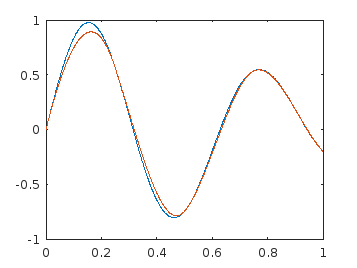
\includegraphics[width=0.8\textwidth]{q4b}
    \caption{Side by side comparison of interpolated (orange) vs original (blue) function.}
    \label{fig:q4b}
\end{figure}

{\medskip\noindent\bf Question 4c.} This question isn't actually asking anything specific, so I'm interpreting this to be asking me to implement it in Matlab. Here is the code used, and a plot of the estimated vs. actual derivative for interpolation over 15 points can be seen in figure \ref{fig:4c}.

\begin{lstlisting}
x = linspace(0, 1, 5);

y = sin(10*x) .* exp(-x.^2);
yp = 10*cos(10*x) .* exp(-x.^2) - 2*x.*sin(10*x) .* exp(-x.^2);

xi = [0.4];

x_dense = linspace(0, 1, 500);
y_dense = sin(10*x_dense) .* exp(-x_dense.^2);
h_dense = hermite(x, y, yp, x_dense);
yp_dense = 10*cos(10*x_dense) .* exp(-x_dense.^2) - 2*x_dense.*sin(10*x_dense) .* exp(-x_dense.^2);

x_approx = x;
y_approx = y;
yp_approx = zeros(length(x_approx),1);
for i = 2:length(x_approx) - 1
    f01 = (y_approx(i)-y_approx(i-1))/(x_approx(i)-x_approx(i-1));
    f12 = (y_approx(i+1)-y_approx(i))/(x_approx(i+1)-x_approx(i));
    f012 = (f12-f01)/(x_approx(i+1)-x_approx(i-1));
    yp_approx(i) = f01+f012*(x_approx(i)-x_approx(i-1));
    if i == 2
        yp_approx(1) = f01+f012*(-x_approx(i)+x_approx(i-1));
    end
    if i == length(x_approx)-1
        yp_approx(end) = f01+f012*(2*x_approx(i+1)-x_approx(i)-x_approx(i-1));
    end
end

plot(x_dense, yp_dense, x_approx, yp_approx);


\end{lstlisting}

\begin{figure}[htpb]
    \centering
    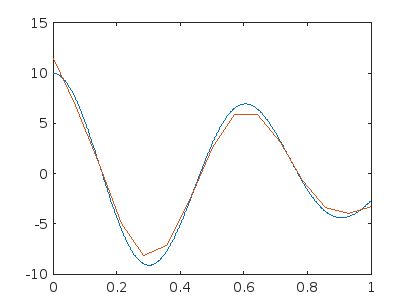
\includegraphics[width=0.8\textwidth]{q4c}
    \caption{Estimated (orange) vs actual (blue) derivative using method from question 3.}
    \label{fig:q4c}
\end{figure}

{\medskip\noindent\bf Question 4d.} This is the routine constructed:

\begin{lstlisting}
function out = pchip_custom(x, y, xq)
    yp = zeros(length(x),1);
    for i = 2:length(x) - 1
        alpha = (2*x(i+1)-x(i)-x(i-1))/3/(x(i+1)-x(i-1));
        f01 = (y(i)-y(i-1))/(x(i)-x(i-1));
        f12 = (y(i+1)-y(i))/(x(i+1)-x(i));
        f012 = (f12-f01)/(x(i+1)-x(i-1));
        % yp(i) = f01+f012*(x(i)-x(i-1));
        if f01*f12 > 0
            yp(i)=f01*f12/(alpha*f12+(1-alpha)*f01);
        else
            yp(i)=0;
        end
        if i == 2
            yp(1) = f01+f012*(-x(i)+x(i-1));
        end
        if i == length(x)-1
            yp(end) = f01+f012*(2*x(i+1)-x(i)-x(i-1));
        end
    end
    out = hermite(x, y, yp, xq);
end
\end{lstlisting}

{\medskip\noindent\bf Question 4e.} See table \ref{tab:4e} and figure \ref{fig:4e}. Here is the full code:

\begin{table}[htpb]
    \centering
    \caption{Values for various interpolation techniques.}
    \label{tab:4e}
    \begin{tabular}{|c|c|c|}
        \hline
        &$N=8$&$N=10$\\
        \hline
        $f(0.4)$&-0.6449&-0.6449\\
        \hline
        $h_{\text{quadratic }f'}(0.4)$&-0.63812&-0.6243\\
        \hline
        $\text{pchip}(0.4)$&-0.6787&-0.6443\\
        \hline
    \end{tabular}
\end{table}

\begin{figure}[htpb]
    \centering
    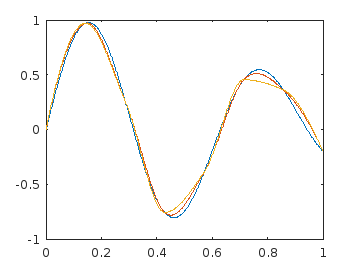
\includegraphics[width=0.8\textwidth]{q4e-8}
    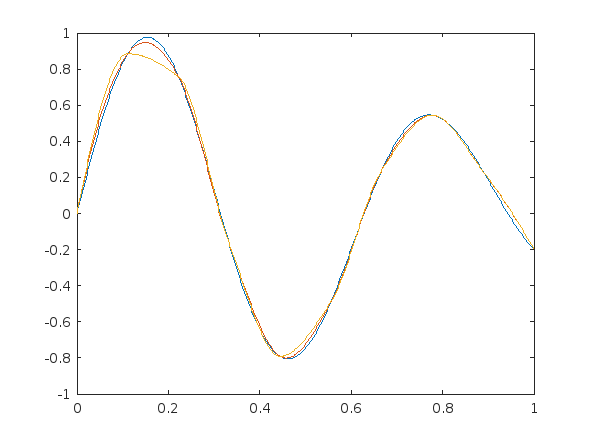
\includegraphics[width=0.8\textwidth]{q4e-10}
    \caption{Graphs for N=8 (top) and N=10 (bottom). The blue is the underlying function, orange is with the derivatives estimated quadratically and yellow is custom pchip.}
    \label{fig:4e}
\end{figure}

\begin{lstlisting}
x = linspace(0, 1, 8);

y = sin(10*x) .* exp(-x.^2);
yp = 10*cos(10*x) .* exp(-x.^2) - 2*x.*sin(10*x) .* exp(-x.^2);

xi = [0.4];


x_dense = linspace(0, 1, 500);
y_dense = sin(10*x_dense) .* exp(-x_dense.^2);
h_dense = hermite(x, y, yp, x_dense);
yp_dense = 10*cos(10*x_dense) .* exp(-x_dense.^2) - 2*x_dense.*sin(10*x_dense) .* exp(-x_dense.^2);

x_approx = x;
y_approx = y;
yp_approx = zeros(length(x_approx),1);
for i = 2:length(x_approx) - 1
    f01 = (y_approx(i)-y_approx(i-1))/(x_approx(i)-x_approx(i-1));
    f12 = (y_approx(i+1)-y_approx(i))/(x_approx(i+1)-x_approx(i));
    f012 = (f12-f01)/(x_approx(i+1)-x_approx(i-1));
    yp_approx(i) = f01+f012*(x_approx(i)-x_approx(i-1));
    if i == 2
        yp_approx(1) = f01+f012*(-x_approx(i)+x_approx(i-1));
    end
    if i == length(x_approx)-1
        yp_approx(end) = f01+f012*(2*x_approx(i+1)-x_approx(i)-x_approx(i-1));
    end
end

h = hermite(x, y, yp_approx, xi);
f = sin(10*xi) .* exp(-xi.^2);
p = pchip_custom(x, y, xi);

display(h)
display(p)

% plot(x_dense, y_dense, x_dense, h, x_dense, p);

% plot(x_dense, yp_dense, x_approx, yp_approx);

function out = pchip_custom(x, y, xq)
    yp = zeros(length(x),1);
    for i = 2:length(x) - 1
        alpha = (2*x(i+1)-x(i)-x(i-1))/3/(x(i+1)-x(i-1));
        f01 = (y(i)-y(i-1))/(x(i)-x(i-1));
        f12 = (y(i+1)-y(i))/(x(i+1)-x(i));
        f012 = (f12-f01)/(x(i+1)-x(i-1));
        % yp(i) = f01+f012*(x(i)-x(i-1));
        if f01*f12 > 0
            yp(i)=f01*f12/(alpha*f12+(1-alpha)*f01);
        else
            yp(i)=0;
        end
        if i == 2
            yp(1) = f01+f012*(-x(i)+x(i-1));
        end
        if i == length(x)-1
            yp(end) = f01+f012*(2*x(i+1)-x(i)-x(i-1));
        end
    end
    out = hermite(x, y, yp, xq);
end

function y_sample = hermite(x, y, yp, xi)
    y_sample = zeros(length(xi), 1);
    for i = 1:length(xi)
        x_cur = xi(i);
        
        for j = 1:length(x) - 1
            if x_cur >= x(j) && x_cur <= x(j + 1)
                break;
            end
        end
        
        delta = x(j+1) - x(j);
        t = (x_cur - x(j)) / delta;
        
        h00 = (1 + 2*t) * (1 - t)^2;
        h10 = t * (1 - t)^2;
        h01 = t^2 * (3 - 2*t);
        h11 = t^2 * (t - 1);
        
        y_sample(i) = h00 * y(j) + h10 * delta * yp(j) + h01 * y(j+1) + h11 * delta * yp(j+1);
    end
end
\end{lstlisting}


\end{document}
